
\includegraphics[height=1.25cm]{images/pictograms/benchmark}

\includegraphics[height=1.25cm]{images/pictograms/under_construction}

\includegraphics[height=1.25cm]{images/pictograms/tools}

\includegraphics[height=1.25cm]{images/pictograms/FEM}

%%%%%%%%%%%%%%%%%%%%%%%%%%%%%%%%%%%%%%%%%%%%%%%%%%%%%%%%%%%%%%%%%%%%%%%%%%%%%%%%%%%%%%%%%%%%%%%%%%%

\begin{flushright} {\tiny {\color{gray} python\_codes/fieldstone\_151/text.tex}} \end{flushright}

\lstinputlisting[language=bash,basicstyle=\small]{python_codes/fieldstone_151/keywords.key}

\par\noindent\rule{\textwidth}{0.4pt}

\begin{center}
\inpython
{\small Code: \url{https://github.com/cedrict/fieldstone/tree/master/python_codes/fieldstone_151}}
\end{center}

\par\noindent\rule{\textwidth}{0.4pt}

%%%%%%%%%%%%%%%%%%%%%%%%%%%%%%%%%%%%%%%%%%%%%%%%%%%%%%%%%%%%%%%%%%%%%%%%%%%%%%%%%%%%%%%%%%%%%%%%%%%


This \stone builds on \stone~\ref{f33} in the sense that in \stone~\ref{f33} free slip boundary conditions 
were implemented and tested on an annulus discretised by means of \QonePzero elements. 
We here implement and test the implementation of such boundary conditions on an annulus discretised
by means of \QtwoQone elements.

As far as I know, there are three ways to implemenent these boundary conditions:
\begin{itemize}
\item the rotating method, \ref{MMM-ss:fsbc_annulus} 
\item constraints applied to elemental matrix
\item constraints via Lagrange multipliers
\end{itemize}



\begin{center}
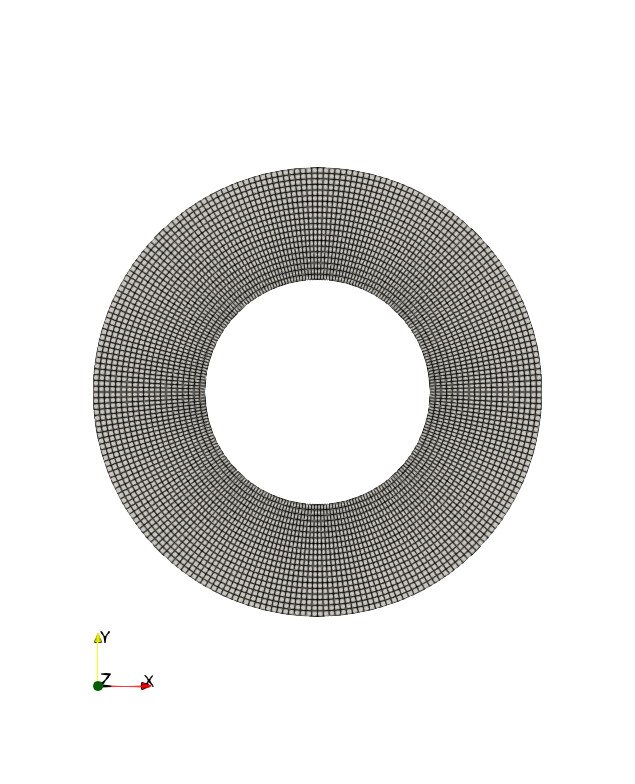
\includegraphics[width=5cm]{./python_codes/fieldstone_151/images/mesh}
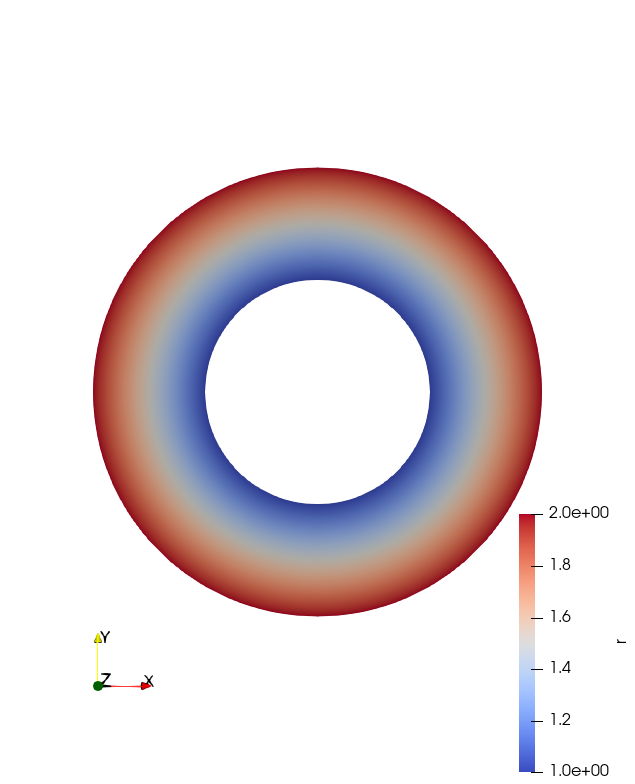
\includegraphics[width=5cm]{./python_codes/fieldstone_151/images/r}
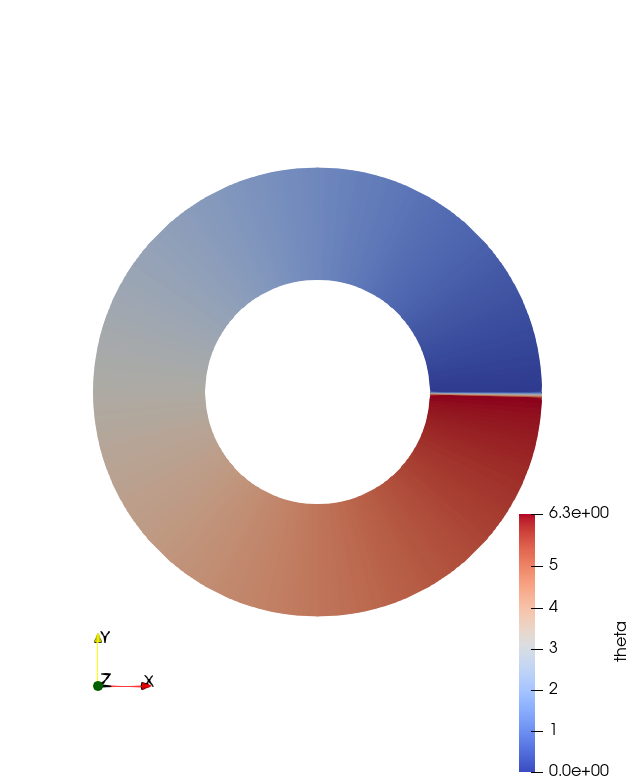
\includegraphics[width=5cm]{./python_codes/fieldstone_151/images/theta}
\end{center}


Goal: 
\begin{itemize}
\item test b.c algorithms
\item straight edge elts vs curved ones.
\end{itemize}

Todo:
remove nnp
proper surface integral for p normalisation

%%%%%%%%%%%%%%%%%%%%%%%%%%%%%%%%%%%%%%%%%%%%%%%%%%%%%%%%%%%%%
\section*{method 1: rotating elemental matrices}

%%%%%%%%%%%%%%%%%%%%%%%%%%%%%%%%%%%%%%%%%%%%%%%%%%%%%%%%%%%%%
\section*{method 2: constraints applied to elemental matrix}

\[
\left(
\begin{array}{cc}
\K_e & \G_e \\
\G_e^T & 0
\end{array}
\right)
\cdot
\left(
\begin{array}{c}
\vec{V} \\
\vec{P}
\end{array}
\right)
=\left(
\begin{array}{c}
\vec{f} \\ \vec{h}
\end{array}
\right)
\]
Let us assume that node 2 is on the boundary and we therefore wish to 
impose $\vec{v}_2\cdot \vec{n}=0$, or $u_2 n_x + v_2 n_y =0$.

The equation above writes (for simplicity we take $m_v=4$ and $m_p=3$ which does not correspond to a real FE pair) with $K_e$ of size 8x8 and $G_e$ of size 8x3 in 2D:
{\small
\[
\begin{array}{ccccccccccccc}
K_{11} u_1 &+ K_{12} v_1 &+ K_{13} u_2 &+ K_{14} v_2 &+ K_{15} u_3 &+ K_{16} v_3 &+ K_{17}u_4  &+ K_{18}v_4  
&+ G_{11}p_1 &+ G_{12} p_2 &+ G_{13} p_3 & =  f_1 \\
K_{21} u_1 &+ K_{22} v_1 &+ K_{23} u_2 &+ K_{24} v_2 &+ K_{25} u_3 &+ K_{26} v_3 &+ K_{27}u_4  &+ K_{28}v_4  
&+ G_{21}p_1 &+ G_{22} p_2 &+ G_{23} p_3 & =  f_2 \\
K_{31} u_1 &+ K_{32} v_1 &+ K_{33} u_2 &+ K_{34} v_2 &+ K_{35} u_3 &+ K_{36} v_3 &+ K_{37}u_4  &+ K_{38}v_4  
&+ G_{31}p_1 &+ G_{32} p_2 &+ G_{33} p_3 & =  f_3 \\
K_{41} u_1 &+ K_{42} v_1 &+ K_{43} u_2 &+ K_{44} v_2 &+ K_{45} u_3 &+ K_{46} v_3 &+ K_{47}u_4  &+ K_{48}v_4  
&+ G_{41}p_1 &+ G_{42} p_2 &+ G_{43} p_3 & =  f_4 \\
K_{51} u_1 &+ K_{52} v_1 &+ K_{53} u_2 &+ K_{54} v_2 &+ K_{55} u_3 &+ K_{56} v_3 &+ K_{57}u_4  &+ K_{58}v_4  
&+ G_{51}p_1 &+ G_{52} p_2 &+ G_{53} p_3 & =  f_5 \\
K_{61} u_1 &+ K_{62} v_1 &+ K_{63} u_2 &+ K_{64} v_2 &+ K_{65} u_3 &+ K_{66} v_3 &+ K_{67}u_4  &+ K_{68}v_4  
&+ G_{61}p_1 &+ G_{62} p_2 &+ G_{63} p_3 & =  f_6 \\
K_{71} u_1 &+ K_{72} v_1 &+ K_{73} u_2 &+ K_{74} v_2 &+ K_{75} u_3 &+ K_{76} v_3 &+ K_{77}u_4  &+ K_{78}v_4  
&+ G_{71}p_1 &+ G_{72} p_2 &+ G_{73} p_3 & =  f_7 \\
K_{81} u_1 &+ K_{82} v_1 &+ K_{83} u_2 &+ K_{84} v_2 &+ K_{85} u_3 &+ K_{86} v_3 &+ K_{87}u_4  &+ K_{88}v_4  
&+ G_{81}p_1 &+ G_{82} p_2 &+ G_{83} p_3 & =  f_8 \\
G_{11}u_1 &+ G_{21}v_1 &+ G_{31}u_2 &+ G_{41}v_2 &+ G_{51}u_3 &+ G_{61}v_3 &+ G_{71}u_4 &+ G_{81}v_4 &+0&+0&+0&= h_1 \\
G_{12}u_1 &+ G_{22}v_1 &+ G_{32}u_2 &+ G_{42}v_2 &+ G_{52}u_3 &+ G_{62}v_3 &+ G_{72}u_4 &+ G_{82}v_4 &+0&+0&+0&= h_2 \\
G_{13}u_1 &+ G_{23}v_1 &+ G_{33}u_2 &+ G_{43}v_2 &+ G_{53}u_3 &+ G_{63}v_3 &+ G_{73}u_4 &+ G_{83}v_4 &+0&+0&+0&= h_3
\end{array}
\]
}
We must now find a way to include the contraint above in these equations.
Typically we usually have $v_2=v_{bc}$ and the system above is transformed as follows
{\small
\[
\begin{array}{lllllllllllll}
K_{11} u_1 &+ K_{12} v_1 &+ K_{13} u_2 &+ 0 &+ K_{15} u_3 &+ K_{16} v_3 &+ K_{17}u_4  &+ K_{18}v_4  
&+ G_{11}p_1 &+ G_{12} p_2 &+ G_{13} p_3 & =  f_1 -K_{14} v_{bc}\\
K_{21} u_1 &+ K_{22} v_1 &+ K_{23} u_2 &+ 0 &+ K_{25} u_3 &+ K_{26} v_3 &+ K_{27}u_4  &+ K_{28}v_4  
&+ G_{21}p_1 &+ G_{22} p_2 &+ G_{23} p_3 & =  f_2 -K_{24} v_{bc}\\
K_{31} u_1 &+ K_{32} v_1 &+ K_{33} u_2 &+ 0 &+ K_{35} u_3 &+ K_{36} v_3 &+ K_{37}u_4  &+ K_{38}v_4  
&+ G_{21}p_1 &+ G_{32} p_2 &+ G_{33} p_3 & =  f_3 -K_{34} v_{bc}\\
0  &+ 0  &+ 0  &+ K_{44} v_2 &+ 0 &+ 0 &+ 0  &+ 0  
&+ 0 &+ 0 &+ 0 & = & K_{44}v_{bc} \\
K_{51} u_1 &+ K_{52} v_1 &+ K_{53} u_2 &+ 0 &+ K_{55} u_3 &+ K_{56} v_3 &+ K_{57}u_4  &+ K_{58}v_4  
&+ G_{21}p_1 &+ G_{52} p_2 &+ G_{53} p_3 & =  f_5 -K_{54} v_{bc}\\
K_{61} u_1 &+ K_{62} v_1 &+ K_{63} u_2 &+ 0 &+ K_{65} u_3 &+ K_{66} v_3 &+ K_{67}u_4  &+ K_{68}v_4  
&+ G_{21}p_1 &+ G_{62} p_2 &+ G_{63} p_3 & =  f_6 -K_{64} v_{bc}\\
K_{71} u_1 &+ K_{72} v_1 &+ K_{73} u_2 &+ 0 &+ K_{75} u_3 &+ K_{76} v_3 &+ K_{77}u_4  &+ K_{78}v_4  
&+ G_{21}p_1 &+ G_{72} p_2 &+ G_{73} p_3 & =  f_7 -K_{74} v_{bc}\\
K_{81} u_1 &+ K_{82} v_1 &+ K_{83} u_2 &+ 0 &+ K_{85} u_3 &+ K_{86} v_3 &+ K_{87}u_4  &+ K_{88}v_4  
&+ G_{21}p_1 &+ G_{82} p_2 &+ G_{83} p_3 & =  f_8 -K_{84} v_{bc}\\
G_{11}u_1 &+ G_{21}v_1 &+ G_{31}u_2 &+ 0 &+ G_{51}u_3 &+ G_{61}v_3 &+ G_{71}u_4 &+ G_{81}v_4 &+0&+0&+0&= h_1 -G_{41}v_{bc}\\
G_{12}u_1 &+ G_{22}v_1 &+ G_{32}u_2 &+ 0 &+ G_{52}u_3 &+ G_{62}v_3 &+ G_{72}u_4 &+ G_{82}v_4 &+0&+0&+0&= h_2 -G_{42}v_{bc}\\
G_{13}u_1 &+ G_{23}v_1 &+ G_{33}u_2 &+ 0 &+ G_{53}u_3 &+ G_{63}v_3 &+ G_{73}u_4 &+ G_{83}v_4 &+0&+0&+0&= h_3 -G_{43}v_{bc}
\end{array}
\]
}
This approach yields an elemental Stokes matrix that is still strictly symmetric. Since we only build $G_{e}$ (and not $G_e^T$) in the code then zeroing a line in $G_e$ means zeroing a line in $G_e^T$ so the approach above reconciles this pb.

If $v_{bc}=0$ then we obtain
{\small
\[
\begin{array}{lllllllllllll}
K_{11} u_1 &+ K_{12} v_1 &+ K_{13} u_2 &+ 0 &+ K_{15} u_3 &+ K_{16} v_3 &+ K_{17}u_4  &+ K_{18}v_4  
&+ G_{11}p_1 &+ G_{12} p_2 &+ G_{13} p_3 & =  f_1 \\
K_{21} u_1 &+ K_{22} v_1 &+ K_{23} u_2 &+ 0 &+ K_{25} u_3 &+ K_{26} v_3 &+ K_{27}u_4  &+ K_{28}v_4  
&+ G_{21}p_1 &+ G_{22} p_2 &+ G_{23} p_3 & =  f_2 \\
K_{31} u_1 &+ K_{32} v_1 &+ K_{33} u_2 &+ 0 &+ K_{35} u_3 &+ K_{36} v_3 &+ K_{37}u_4  &+ K_{38}v_4  
&+ G_{21}p_1 &+ G_{32} p_2 &+ G_{33} p_3 & =  f_3 \\
0  &+ 0  &+ 0  &+ K_{44} v_2 &+ 0 &+ 0 &+ 0  &+ 0  
&+ 0 &+ 0 &+ 0 & =  0 \\
K_{51} u_1 &+ K_{52} v_1 &+ K_{53} u_2 &+ 0 &+ K_{55} u_3 &+ K_{56} v_3 &+ K_{57}u_4  &+ K_{58}v_4  
&+ G_{21}p_1 &+ G_{52} p_2 &+ G_{53} p_3 & =  f_5 \\
K_{61} u_1 &+ K_{62} v_1 &+ K_{63} u_2 &+ 0 &+ K_{65} u_3 &+ K_{66} v_3 &+ K_{67}u_4  &+ K_{68}v_4  
&+ G_{21}p_1 &+ G_{62} p_2 &+ G_{63} p_3 & =  f_6 \\
K_{71} u_1 &+ K_{72} v_1 &+ K_{73} u_2 &+ 0 &+ K_{75} u_3 &+ K_{76} v_3 &+ K_{77}u_4  &+ K_{78}v_4  
&+ G_{21}p_1 &+ G_{72} p_2 &+ G_{73} p_3 & =  f_7 \\
K_{81} u_1 &+ K_{82} v_1 &+ K_{83} u_2 &+ 0 &+ K_{85} u_3 &+ K_{86} v_3 &+ K_{87}u_4  &+ K_{88}v_4  
&+ G_{21}p_1 &+ G_{82} p_2 &+ G_{83} p_3 & =  f_8 \\
G_{11}u_1 &+ G_{21}v_1 &+ G_{31}u_2 &+ 0 &+ G_{51}u_3 &+ G_{61}v_3 &+ G_{71}u_4 &+ G_{81}v_4 &+0&+0&+0&= h_1 \\
G_{12}u_1 &+ G_{22}v_1 &+ G_{32}u_2 &+ 0 &+ G_{52}u_3 &+ G_{62}v_3 &+ G_{72}u_4 &+ G_{82}v_4 &+0&+0&+0&= h_2 \\
G_{13}u_1 &+ G_{23}v_1 &+ G_{33}u_2 &+ 0 &+ G_{53}u_3 &+ G_{63}v_3 &+ G_{73}u_4 &+ G_{83}v_4 &+0&+0&+0&= h_3 
\end{array}
\]
}




Let us now turn to free slip and start with $v_2=-u_2 n_x/n_y$. Then we could write:
{\small
\[
\begin{array}{lllllllllllll}
K_{11} u_1 &+ K_{12} v_1 &+ (K_{13}-\frac{n_x}{n_y}K_{14}) u_2 &+ 0 &+ K_{15} u_3 &+ K_{16} v_3 &+ K_{17}u_4  &+ K_{18}v_4  
&+ G_{11}p_1 &+ G_{12} p_2 &+ G_{13} p_3 & =  f_1 \\
K_{21} u_1 &+ K_{22} v_1 &+ (K_{23}-\frac{n_x}{n_y}K_{24}) u_2 &+ 0 &+ K_{25} u_3 &+ K_{26} v_3 &+ K_{27}u_4  &+ K_{28}v_4  
&+ G_{21}p_1 &+ G_{22} p_2 &+ G_{23} p_3 & =  f_2 \\
K_{31} u_1 &+ K_{32} v_1 &+ (K_{33}-\frac{n_x}{n_y}K_{34}) u_2 &+ 0 &+ K_{35} u_3 &+ K_{36} v_3 &+ K_{37}u_4  &+ K_{38}v_4  
&+ G_{31}p_1 &+ G_{32} p_2 &+ G_{33} p_3 & =  f_3 \\
0 &+ 0 & +K_{44}\frac{n_x}{n_y} u_2 &+ K_{44} v_2 &+ 0 &+ 0 &+ 0  &+ 0  
&+ 0 &+ 0 &+ 0 & =  0 \\
K_{51} u_1 &+ K_{52} v_1 &+ (K_{53}-\frac{n_x}{n_y}K_{54}) u_2 &+ 0 &+ K_{55} u_3 &+ K_{56} v_3 &+ K_{57}u_4  &+ K_{58}v_4  
&+ G_{51}p_1 &+ G_{52} p_2 &+ G_{53} p_3 & =  f_5 \\
K_{61} u_1 &+ K_{62} v_1 &+ (K_{63}-\frac{n_x}{n_y}K_{64}) u_2 &+ 0 &+ K_{65} u_3 &+ K_{66} v_3 &+ K_{67}u_4  &+ K_{68}v_4  
&+ G_{61}p_1 &+ G_{62} p_2 &+ G_{63} p_3 & =  f_6 \\
K_{71} u_1 &+ K_{72} v_1 &+ (K_{73}-\frac{n_x}{n_y}K_{74}) u_2 &+ 0 &+ K_{75} u_3 &+ K_{76} v_3 &+ K_{77}u_4  &+ K_{78}v_4  
&+ G_{71}p_1 &+ G_{72} p_2 &+ G_{73} p_3 & =  f_7 \\
K_{81} u_1 &+ K_{82} v_1 &+ (K_{83}-\frac{n_x}{n_y}K_{84}) u_2 &+ 0 &+ K_{85} u_3 &+ K_{86} v_3 &+ K_{87}u_4  &+ K_{88}v_4  
&+ G_{81}p_1 &+ G_{82} p_2 &+ G_{83} p_3 & =  f_8 \\
G_{11}u_1 &+ G_{21}v_1 &+ (G_{31}-\frac{n_x}{n_y}G_{41})u_2 &+0  &+ G_{51}u_3 &+ G_{61}v_3 &+ G_{71}u_4 &+ G_{81}v_4 &+0&+0&+0&= h_1 \\
G_{12}u_1 &+ G_{22}v_1 &+ (G_{32}-\frac{n_x}{n_y}G_{42})u_2 &+0  &+ G_{52}u_3 &+ G_{62}v_3 &+ G_{72}u_4 &+ G_{82}v_4 &+0&+0&+0&= h_2 \\
G_{13}u_1 &+ G_{23}v_1 &+ (G_{33}-\frac{n_x}{n_y}G_{43})u_2 &+0  &+ G_{53}u_3 &+ G_{63}v_3 &+ G_{73}u_4 &+ G_{83}v_4 &+0&+0&+0&= h_3
\end{array}
\]
}
which is not very useful since the symmetry has been destroyed. Note that when $n_x\rightarrow 0$ 
then we recover the system above.

May be the simplest approach is then to do
{\small
\[
\begin{array}{lllllllllllll}
K_{11} u_1 &+ K_{12} v_1 &+ K_{13} u_2 &+ K_{14} v_2 &+ K_{15} u_3 &+ K_{16} v_3 &+ K_{17}u_4  &+ K_{18}v_4  
&+ G_{11}p_1 &+ G_{12} p_2 &+ G_{13} p_3 & =  f_1 \\
K_{21} u_1 &+ K_{22} v_1 &+ K_{23} u_2 &+ K_{24} v_2 &+ K_{25} u_3 &+ K_{26} v_3 &+ K_{27}u_4  &+ K_{28}v_4  
&+ G_{21}p_1 &+ G_{22} p_2 &+ G_{23} p_3 & =  f_2 \\
K_{31} u_1 &+ K_{32} v_1 &+ K_{33} u_2 &+ K_{34} v_2 &+ K_{35} u_3 &+ K_{36} v_3 &+ K_{37}u_4  &+ K_{38}v_4  
&+ G_{31}p_1 &+ G_{32} p_2 &+ G_{33} p_3 & =  f_3 \\
0 &+ 0 & +K_{44}\frac{n_x}{n_y} u_2 &+ K_{44} v_2 &+ 0 &+ 0 &+ 0  &+ 0  
&+ 0 &+ 0 &+ 0 & =  0 \\
K_{51} u_1 &+ K_{52} v_1 &+ K_{53} u_2 &+ K_{54} v_2 &+ K_{55} u_3 &+ K_{56} v_3 &+ K_{57}u_4  &+ K_{58}v_4  
&+ G_{51}p_1 &+ G_{52} p_2 &+ G_{53} p_3 & =  f_5 \\
K_{61} u_1 &+ K_{62} v_1 &+ K_{63} u_2 &+ K_{64} v_2 &+ K_{65} u_3 &+ K_{66} v_3 &+ K_{67}u_4  &+ K_{68}v_4  
&+ G_{61}p_1 &+ G_{62} p_2 &+ G_{63} p_3 & =  f_6 \\
K_{71} u_1 &+ K_{72} v_1 &+ K_{73} u_2 &+ K_{74} v_2 &+ K_{75} u_3 &+ K_{76} v_3 &+ K_{77}u_4  &+ K_{78}v_4  
&+ G_{71}p_1 &+ G_{72} p_2 &+ G_{73} p_3 & =  f_7 \\
K_{81} u_1 &+ K_{82} v_1 &+ K_{83} u_2 &+ K_{84} v_2 &+ K_{85} u_3 &+ K_{86} v_3 &+ K_{87}u_4  &+ K_{88}v_4  
&+ G_{81}p_1 &+ G_{82} p_2 &+ G_{83} p_3 & =  f_8 \\
G_{11}u_1 &+ G_{21}v_1 &+ G_{31}u_2 &+ G_{41}v_2 &+ G_{51}u_3 &+ G_{61}v_3 &+ G_{71}u_4 &+ G_{81}v_4 &+0&+0&+0&= h_1 \\
G_{12}u_1 &+ G_{22}v_1 &+ G_{32}u_2 &+ G_{42}v_2 &+ G_{52}u_3 &+ G_{62}v_3 &+ G_{72}u_4 &+ G_{82}v_4 &+0&+0&+0&= h_2 \\
G_{13}u_1 &+ G_{23}v_1 &+ G_{33}u_2 &+ G_{43}v_2 &+ G_{53}u_3 &+ G_{63}v_3 &+ G_{73}u_4 &+ G_{83}v_4 &+0&+0&+0&= h_3
\end{array}
\]
}
but it means that after imposing the b.c. I end up with a system like

\[
\left(
\begin{array}{cc}
K_e & G_1 \\
G_1^T & 0
\end{array}
\right)
\cdot
\left(
\begin{array}{c}
\vec{V} \\
\vec{P}
\end{array}
\right)
=\left(
\begin{array}{c}
\vec{f} \\ \vec{h}
\end{array}
\right)
\]



\newpage
%%%%%%%%%%%%%%%%%%%%%%%%%%%%%%%%%%%%%%%%%%%%%%%%%%%%%%%%%%%%%%%%%%%%%%%%%%%%%%%%%%%%%%%%%%%%%%%%%%%

In what follows we set $R_1=1$ and $R_2=2$. Unless otherwise specified we also set $\rho=1$
and $\eta=1$. The following tests are such that there is no rotational nullspace.

%%%%%%%%%%%%%%%%%%%%%%%%%%%%%%%%%%%%%%%%%%%
\section*{test \#1: the aquarium - no slip}


%%%%%%%%%%%%%%%%%%%%%%%%%%%%%%%%%%%%%%%%%%%
\section*{test \#2: the aquarium - free slip}


%%%%%%%%%%%%%%%%%%%%%%%%%%%%%%%%%%%%%%%
\section*{test \#3: shearing - no slip}


%%%%%%%%%%%%%%%%%%%%%%%%%%%%%%%%%%%%%%%%%
\section*{test \#4: shearing - free slip}








%%%%%%%%%%%%%%%%%%%%%%%%%%%%%%%%%%%%%%%%%%%%%%%%%%%%%%%%%%%%%%%%%%%%%%%%%%%%%%%%%%%%%%%%%%%%%%%%%%%
\par\noindent\rule{\textwidth}{0.4pt}

\vspace{.5cm}

\begin{center}
\fbox{\begin{minipage}{0.9\textwidth}
{\color{teal}To Do, open questions, future work?}
\begin{itemize}
\item do smthg
\end{itemize}
\end{minipage}}
\end{center}

%%%%%%%%%%%%%%%%%%%%%%%%%%%%%%%%%%%%%%%%%%%%%%%%%%%%%%%%%%%%%%%%%%%%%%%%%%%%%%%%%%%%%%%%%%%%%%%%%%%
\vspace{.5cm}

\Literature:\\
\fullcite{xxxxYY}

